\section{Additional Empirical Results}
\label{sec:additional-results}

\begin{figure}[h]
    \centering
    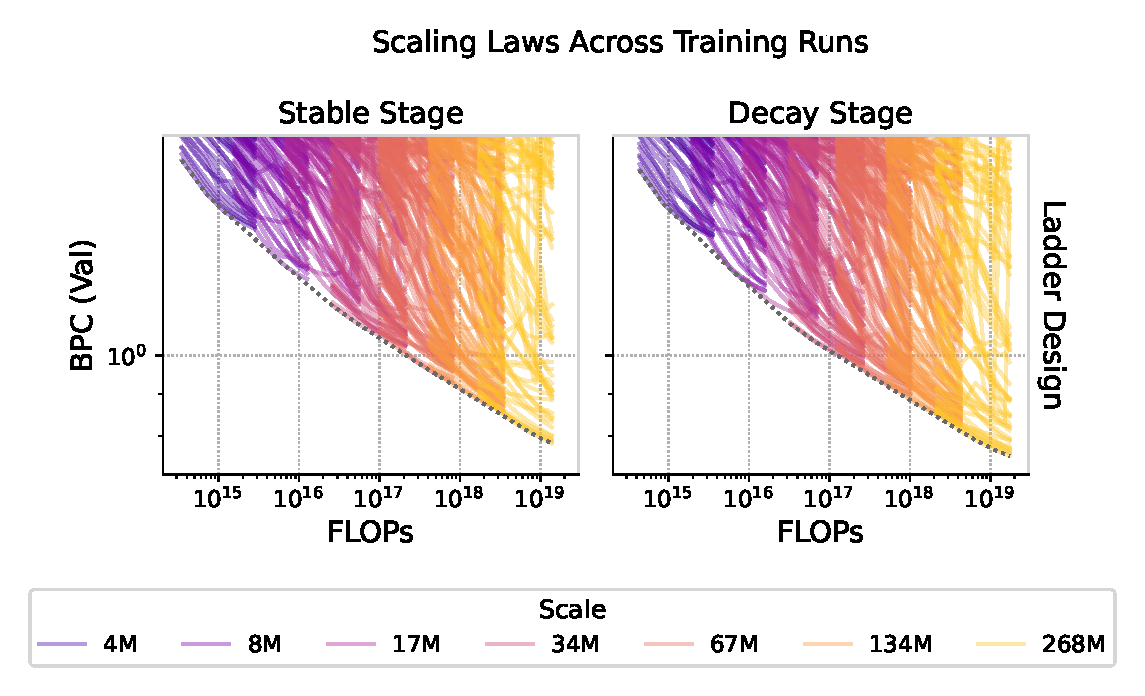
\includegraphics[width=0.68\linewidth]{figures/scaling-laws-on-the-fully-tuned-frontier.pdf}
    \caption{
        \emph{Scaling laws emerge at very small scales, smaller than widely believed; however, hyperparameter tuning becomes critical.} Predictable scaling appears only at the fully tuned frontier. Smaller models are harder to tune, making their scaling laws harder to observe though no less present.
    }
    \label{fig:scaling-laws-at-the-fully-tuned-frontier}
\end{figure}

\begin{figure}[h]
\vspace{-1cm}
    \centering
    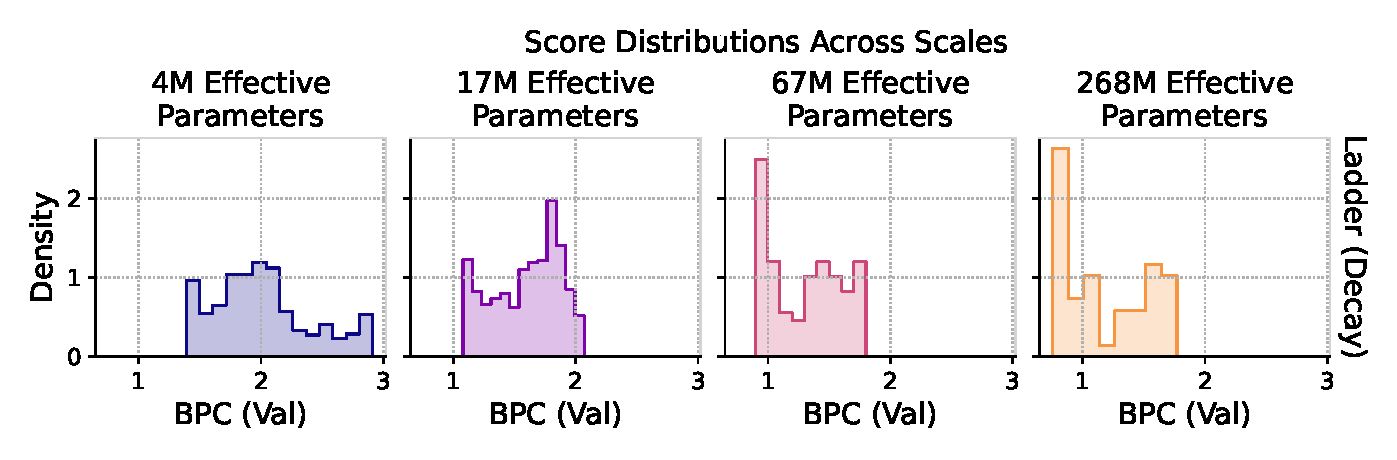
\includegraphics[width=0.7\linewidth]{figures/hyperparameter-sensitivity-decreases-with-scale.pdf}
    \caption{
        \emph{As scale increases, random configurations are more likely to land near the optimum.} We measure the volume of near-optimal configurations by visualizing the distribution over validation scores at the end of training from random search (the best 85\% to avoid divergent runs). As scale grows, the distribution concentrates near the best achievable loss at each scale, with probability mass piling up into a peak. Good configurations fill the space and get easier to find.
    }
    \label{fig:hyperparameter-sensitivity-decreases-with-scale}
\end{figure}

\begin{figure}[h]
\vspace{-1cm}
    \centering
    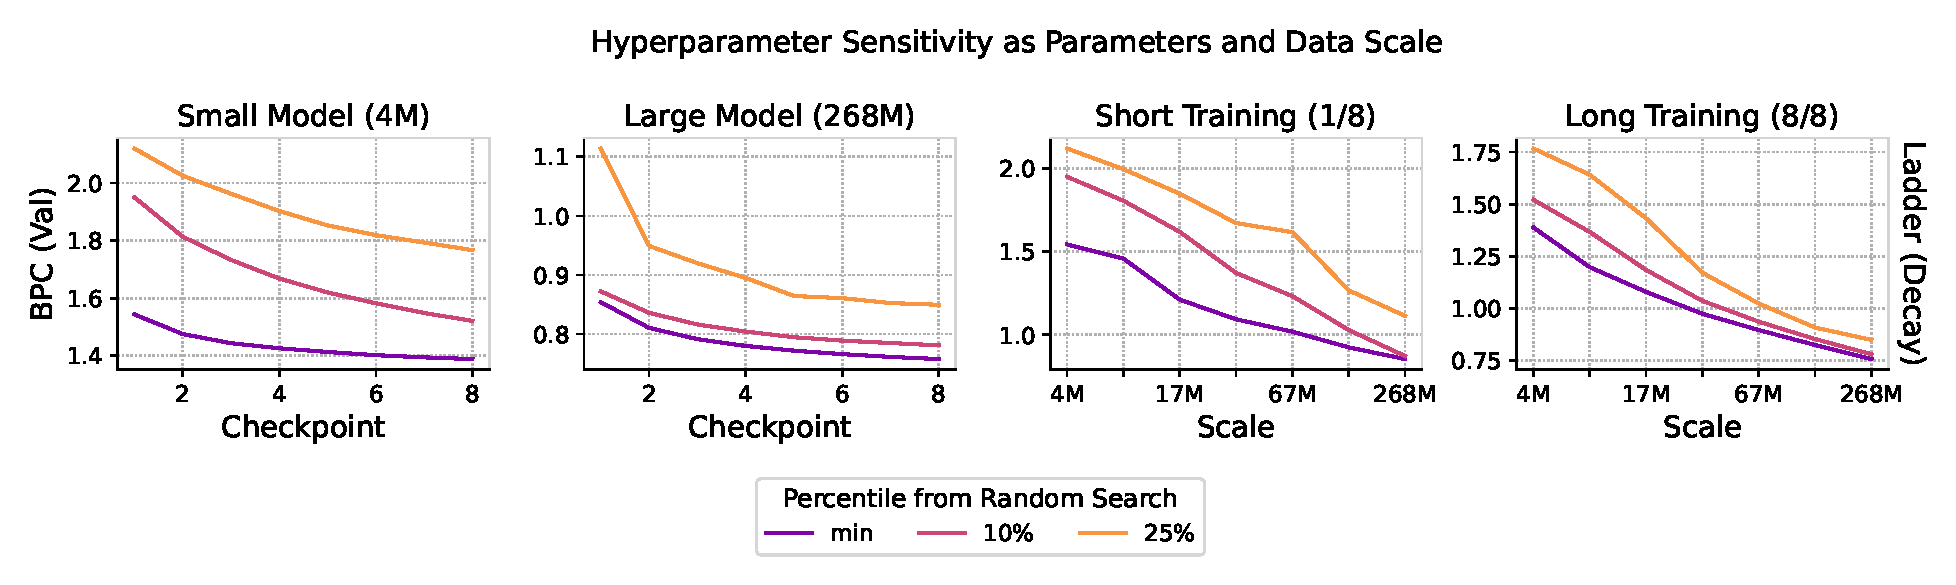
\includegraphics[width=\linewidth]{figures/hyperparameter-sensitivity-decreases-through-both-parameters-and-data.pdf}
    \caption{
        \emph{Hyperparameter sensitivity diminishes through increasing parameters and data together.} We plot the minimum, 10th, and 25th percentile validation losses from random search. The gap from the minimum measures sensitivity. Scaling data with a small model (left) or parameters with short training (middle right) lowers the loss but only slightly cuts the gap. Scaling data with a large model (middle left) or parameters with longer training (right) collapses the gap.
    }
    \label{fig:hyperparameter-sensitivity-decreases-through-both-parameters-and-data}
\end{figure}



% \begin{figure}
%     \centering
%     \begin{minipage}{0.48\textwidth}
%         \centering
%         \includegraphics[width=\textwidth]{figures/effective-hyperparameters-decrease-with-scale.pdf}
%         \caption{
%             \emph{Big models have fewer effective hyperparameters.} The effective hyperparameter count ($\gamma$) is the intrinsic dimension of the hyperparameter loss surface around the optimum. We estimate $\gamma$ by fitting the noisy quadratic to random search results. $\gamma$ drops to 1 as models scale.
%         }
%         \label{fig:effective-hyperparameters-decrease-with-scale}
%     \end{minipage}
%     \hfill
%     \begin{minipage}{0.51\textwidth}
%         \centering
%         \includegraphics[width=\textwidth]{figures/effective-hyperparameters-by-parameters-and-tokens.pdf}
%         \caption{
%             \emph{Parameters, more than data, reduce the effective number of hyperparameters.} The effective hyperparameter count ($\gamma$) is the intrinsic dimension of the hyperparameter loss surface. We estimate $\gamma$ at each parameter--data budget by fitting the noisy quadratic distribution to results from random search. With and without learning rate decay, $\gamma$ trends lower as parameters increase, while increasing data has much less of an effect.
%         }
%         \label{fig:effective-hyperparameters-by-parameters-and-tokens}
%     \end{minipage}
% \end{figure}
